%\documentclass[a4j,twocolumn,uplatex]{jsarticle}
\documentclass[a4j,twocolumn]{jsarticle}

\usepackage[dvipdfmx]{graphicx}
\usepackage{url}
\usepackage{amsmath}
\def\tightlist{\itemsep1pt\parskip0pt\parsep0pt}
\setlength{\textheight}{275mm}
\headheight 5mm
\topmargin -30mm
\textwidth 185mm
\oddsidemargin -15mm
\evensidemargin -15mm
\setlength\textfloatsep{0pt}
\setlength\intextsep{0pt}
\pagestyle{empty}


\begin{document}

\title{command lineによるeditor操作の習熟プログラムの開発}
\author{情報科学科 \hspace{5mm} 27014533 \hspace{5mm} 和田創煕}
\date{}
\maketitle


\section{研究の動機}
最初は西谷によって開発されたshunkuntype(ターミナル上で実行するタイピングソフト)の再開発をテーマにしていたが,タイピングに特化したソフトを開発しても同じようなものがWeb上に大量に配布されており,それ以上の付加価値を持ったソフトを開発しようと考えた.

プログラマにとって作業を効率化する要因としてeditor操作に関しては,


\begin{quotation}
ツールはプログラマ自身の手の延長である.これは他のどのようなソフトウェアツールよりもEditorに対して当てはまる.テキストはできる限り簡単に操作できる必要があり,一つの強力なeditorの習熟は作業の効率化に欠かせない\cite{達人プログラマー}. 
\end{quotation}
と記述されている.西谷研究室ではタイピング,Ruby言語,Emacsによるeditor操作,CUI操作の習熟が作業効率に非常に大きな影響を与えるため習熟を勧めているのでこれらの習熟を目的としたソフトを開発しようと考えた.


\section{editor\_learnerの概要}
本章では,editor\_learnerのメソッドについて説明する.練習用コードはRuby入門の教科書を参考にしている\cite{ruby}.
\subsection{initialize}
各種コマンドを実行した時,自動的に動くメソッドである.作業を行うためのファイルの作成,gemでinstallした先のパスを格納したインスタンス変数の定義がメインである.
\subsection{random\_check}
コマンド実行から終了までの動作の概要は以下の通り.
\begin{enumerate}
\def\labelenumi{\arabic{enumi}.}
\tightlist
\item
用意されたソースコードから1つ選ばれ,question.rbコピーされる.
\item
新しいターミナルが開かれ,question.rbの内容をanswer.rbに写経する.
\item
写経し終えると前のターミナルに戻り"check"とコマンドラインで入力する.
\item
正しければ終了,正しくなければ間違った箇所のみが表示され,再度確認,入力,正誤判定を繰り返す.
\end{enumerate}
\subsection{sequential\_check}
コマンド実行から終了までの動作の概要は以下の通り.
\begin{enumerate}
\def\labelenumi{\arabic{enumi}.}
\tightlist
\item
chapterと問題番号を引数として入力.対応した問題がq.rbにコピーされる.
\item
新しいターミナルが開かれ,写経する.
\item
写経し終えた後の動作は2.2の4番からはrandom\_checkと同じ動作である.
\end{enumerate}
一度写経し終えた問題を再度行う時には,作成されたファイルの削除を行うメソッドが別途用意されている.

\section{他のソフトとの比較}

表1は人気タイピングソフトとeditor\_learnerの利点,欠点とユーザーインタフェースを表にしたものである.

CUIに近いPTYPINGが高評価な理由はコードに関する単語を入力できるという点であった.それに加えてeditor\_learnerはeditor操作やコードの入力,実行ができる.

GUIベースのソフトには継続性に関しては劣る.しかしCUIベースであればキーバインド使用により作業の高速化,効率化が期待される.そのためeditor\_learnerはプログラマ向けの機能を多数有しているソフトである.
\begin{table}[h]
\begin{center}
\caption{人気タイピングソフトとeditor\_learnerの利点,欠点とユーザーインタフェース.\label{sample}}
\vspace{-0.5zh}
\centering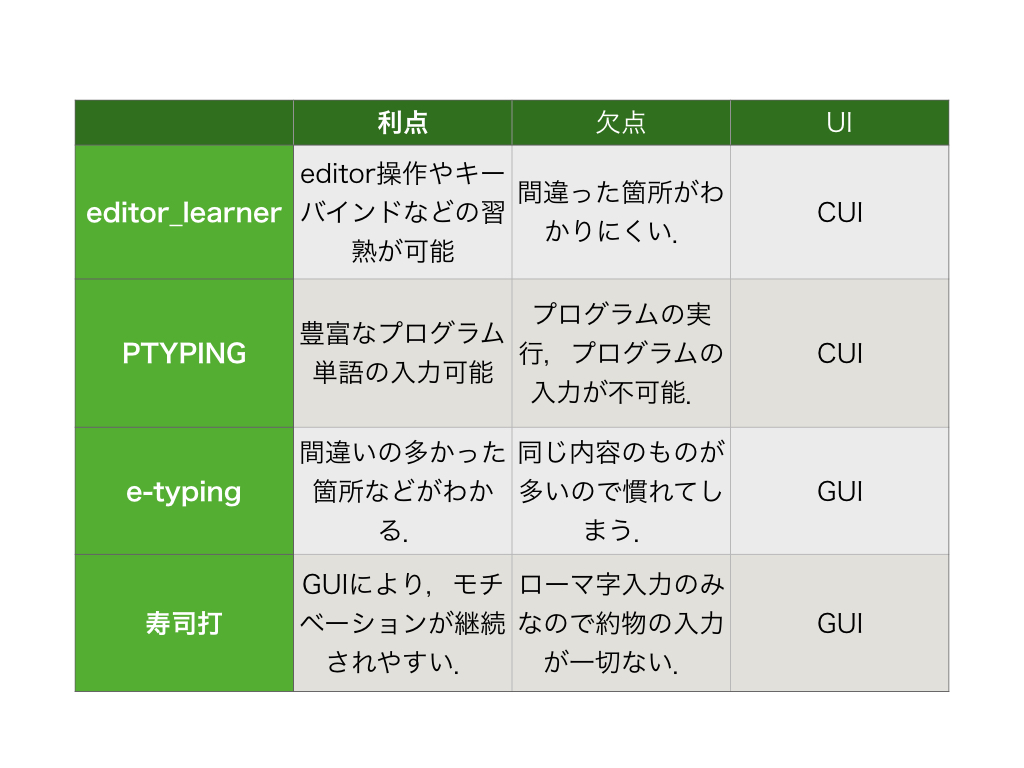
\includegraphics[width=80mm]{../handout/ok/ok.jpeg}
\end{center}

\label{fig:This}
\end{table}
\vspace{-3zh}
\section{終わりに}
editor\_learnerは\{\}や()など約物の入力やカーソル移動,ファイルの開閉,保存などのCUI操作を全てキーバインドで行う.そのため,editor\_learnerはプログラマにとって作業を効率化させるソフトと言え,ソフトの目的に沿った技術の向上が期待される.
\begin{thebibliography}{9}
\bibitem{達人プログラマー} Andrew Hunt, David Thomas, 「達人プログラマー」, (オーム社, 2016年).
\bibitem{ruby} 伊藤淳一, 「プロを目指す人のためのRuby入門」, (技術評論社, 2017年)
\end{thebibliography}


\end{document}